%&latex
%
\documentclass[../template.tex]{subfiles}
\begin{document}

\section{Integrals in $\mathbb{C}$}
\lesson{5}{17/10/19}

\subsection{Fourier Integral}
Recall the \textbf{Fourier transform} of a function $f(x)$:
\begin{align*}
    \mathcal{F}(f(x)) \equiv \tilde{f}(k) \equiv \int_{-\infty}^{+\infty}  e^{-ikx} f(x) \dd{x}
\end{align*} 
The \textit{inverse} Fourier transform is then:
\begin{align*}
    \mathbb{F}^{-1}(\tilde{f}(k)) \equiv \frac{1}{2 \pi} \int_{-\infty}^{+\infty} e^{ikx} \tilde{f}(k)  \dd{k}
\end{align*} 
Note that, by our convention, we will put the $(2 \pi)^{-1}$ normalization factor only in the inverse, and not in the direct Fourier transform.

\begin{itemize}
    \item One simple Fourier transform is that of the $\delta(x)$ distribution:
    \begin{align*}
        \mathbb{F}(\delta(x)) = \int_{-\infty}^{+\infty}  e^{-ikx} \delta(x) \dd{x} = 1
    \end{align*} 
    In fact, we could use this relation to \textit{define} $\delta(x)$:
    \begin{align*}
        \delta(x) \equiv \mathbb{F}^{-1}(1) = \frac{1}{2\pi} \int_{-\infty}^{+\infty}   e^{ikx} \dd{k}
    \end{align*}  
    \item The \textbf{Heaviside function}  is defined as:
    \begin{align*}
        \theta_0(x) = \begin{cases}
            -1 & x<0\\
            \frac{1}{2} & x=0\\
            +1 & x>0 
        \end{cases}    
    \end{align*}
    If we \textit{remove} the middle value, we can write the resulting function $\theta(x)$  in terms of the \textit{sign function}: 
    \begin{align*}
        \operatorname{sign}(x) = \begin{cases}
            1 & x > 0\\
            -1 & < 0
        \end{cases}
    \end{align*}   
    noting that:
    \begin{align*}
        \theta(x) = \frac{1}{2} + \frac{\operatorname{sign}(x)}{2}  
    \end{align*}
    To compute the Fourier transform of $\theta(x)$ we start by differentiating:
    \begin{align*}
        \dv{x} \theta(x) = \dv{x} \frac{\operatorname{sign}(x)}{2} = \delta(x)  
    \end{align*} 
    and then make use of a property of Fourier transforms:
    \begin{align*}
        \mathcal{F}\left(\dv{x} f(x)\right) = ik \tilde{f}(k)
    \end{align*}
    (Prove this as \textbf{exercise})
    leading to:
    \begin{align*}
        \tilde{\theta}(k) &= \frac{1}{ik} \mathcal{F}\left(\dv{x} \theta(x)\right) + \mathcal{F}\left(\frac{1}{2} \right) = \frac{1}{ik} \cdot 1 + \frac{1}{2} \mathcal{F}(1) =\\
        &\underset{(a)}{=}    \frac{1}{ik} + \pi \delta(x) 
    \end{align*}
    (As \textbf{exercise}, prove that $\mathcal{F}(1) = 2\pi \delta(x)$, the result we used in (a)).
\end{itemize}

\subsection{Fresnel integral}
We now introduce a new kind of integral, which will be useful to solve the Schr\"odinger equation after applying a Fourier transform:
\begin{align*}
    i \mathcal{G}(\vec{r},t; \vec{r}\,',t') = \int \frac{\dd[3]{k}}{(2\pi)^3} \exp\left(-\frac{i \hbar}{2m}k^2(t-t') - i \vec{k}(\vec{r}-\vec{r}\,') \right) 
\end{align*}
where $\mathcal{G}$ is the \textit{propagator} (a measure of probability of transition between two positions in a quantum system - will be explained in detail later in the course).\\

\begin{example}
    Consider the following integral:
    \begin{align*}
        I(a,b) = \int_{-\infty}^{+\infty} \frac{\dd{k}}{2 \pi} e^{-iak^2 - ibk} = \frac{1}{(4 \pi a i)^{1/2}} \exp\left(\frac{ib^2}{4a} \right)  \qquad a,b \in \mathbb{R}
    \end{align*}
    Note that $I(a,b)$ is similar to $Z(A,b)$, but it lies in the complex plane.
    \begin{enumerate}
        \item Suppose $a > 0$. We consider a slight \q{nudge} of the imaginary axis by a a small clockwise angle $\epsilon > 0$, that is:
        \begin{align*}
            i_\epsilon = \exp\left(i \left(\frac{\pi}{2} - \epsilon\right)\right) = e^{i 2 \Phi_\epsilon} \qquad \Phi_\epsilon = \frac{\pi}{4} - \frac{\epsilon}{2}    
        \end{align*}     
        We replace $i$ with $i_\epsilon$ in the first exponential term:  
        \begin{align*}
            I_\epsilon(a,b) = \int_{-\infty}^{+\infty} \frac{\dd{k}}{2 \pi} \exp(-a k^2 e^{2i \Phi_\epsilon} - ibk)
        \end{align*}
        Note that $I_\epsilon \to I$ as $\epsilon \to 0$. Also, as:
        \begin{align*}
            \operatorname{Re}(e^{2i \Phi_\epsilon}) = \cos\left(\frac{\pi}{2} - \epsilon \right)  > 0
        \end{align*}  
        $I_\epsilon$ is well defined.\\
        Now, consider the following change of variables:
        \begin{align*}
            k e^{i \Phi_\epsilon} = z \Rightarrow \dd{k} = \dd{z} e^{-i \Phi_\epsilon} 
        \end{align*} 
        and let $b' = e^{-i \Phi_\epsilon} b$ for simplicity. We arrive at:
        \begin{align*}
            I_\epsilon(a,b) = \frac{e^{-i \Phi_\epsilon}}{2 \pi} \int_\gamma e^{-a z^2 - izb'} \dd{z} 
        \end{align*}
        where $\gamma$ is the new path of integration, i.e. a line passing through the origin of the complex plane, forming an angle of $\Phi_\epsilon$ with the real axis.\\
        To solve the complex integral we invoke, as usual, the Cauchy Residual Theorem. For that we need a close path $\Gamma$:
        \begin{itemize}
            \item Start following $\gamma$ 
            \item Follow an arc of circumference $\gamma_+$  to a point $R \gg 0$ on the real axis.
            \item Follow the real axis $\bar{\gamma}_R$  from right to left, up to $-R$
            \item Follow an arc of circumference $\gamma_-$  leading back to $\gamma$    
        \end{itemize}
        \begin{figure}[H]
            \centering
            \includegraphics[width=0.8\textwidth]{Images/path.pdf}
            \caption{Path of the integral\label{fig:path}}
        \end{figure}
        
        So that:
        \begin{align*}
            I_{R,\epsilon} (a,b) = \int_\Gamma \dd{z} e^{-a z^2 - iz b'} = 0
        \end{align*}
        as there are no singularities inside $\Gamma = \gamma \cup \gamma_+ \cup \bar{\gamma}_R \cup \gamma_-$, where:
        \begin{align*}
            \gamma_+ &= \{ z = Re^{i \theta}, \theta \in [0, \Phi_\epsilon]\}\\
            \gamma_- &= \{z = Re^{i \theta}, \theta \in [\pi, \pi + \Phi_\epsilon]\}\\
            \gamma_R &= \{z \in \gamma, |z| \leq R\}\\
            \bar{\gamma}_R &= [-R, R]
        \end{align*} 
        Note that:
        \begin{align*}
            \left|I^{\gamma_+}_{R,\epsilon}\right|  &\xrightarrow[R \to \infty]{}  0\\
            \left|I_{R,\epsilon}^{\gamma_-}\right| & \xrightarrow[R \to \infty]{}  0
        \end{align*}
        In fact:
        \begin{align} \nonumber
            \left|\int_{\gamma_+} e^{-az^2 - ib'z} \dd{z} \right| &= \left| -Ri \int_{\theta = 0}^{\theta= \Phi_\epsilon}\dd{\theta} \exp\left\{i \theta - a R^2 e^{2i \theta} - i R b' e^{i \theta}\right\}
            \right| \leq\\
            & \leq R \int_{0}^{\Phi_\epsilon} \dd{\theta} \exp\left\{ 
            -aR^2 \cos(2 \theta)
            \right\} \left|\exp\left\{ iR b e^{-i \Phi_\epsilon + i \theta}\right \} \right|
            \label{eqn:int-step1}
        \end{align}
        Note that $\cos(2 \theta) >0$, as $2 \theta < \pi/2$. Then:
        \begin{align*}
            (\ref{eqn:int-step1}) \leq R \int_{0}^{\Phi_\epsilon} \dd{\theta} \exp\left \{
            -aR^2 \cos(2 \theta) + Rb \sin(-\Phi_\epsilon + \theta)
            \right\} \leq R e^{-a R^2 \sin \Phi_\epsilon}  \xrightarrow[R \to \infty]{}  0
        \end{align*}  
    
    And the same steps can be repeated for $\gamma_-$.\\
    
    Then:
    \begin{align*}
        I_{\gamma_R} = - I_{\bar{\gamma}_R} = I_{\bar{\gamma}_R^{-1}}
    \end{align*}
    And so:
    \begin{align*}
        I_\epsilon(a,b) &= \frac{1}{2 \pi} e^{-i \Phi_\epsilon} \int_{-\infty}^{+\infty}  e^{-a z^2 - ib'z} \dd{z} \underset{(a)}{=}  \frac{1}{2 \pi} e^{-i \Phi_\epsilon} \sqrt{\frac{\pi}{a}} \exp\left(-\frac{(b')^2}{4a} \right) =\\
        &= (4 \pi a)^{-\frac{1}{2}} e^{-i \Phi_\epsilon} \exp \left(-\frac{(b')^2}{4a} \right)
    \end{align*}
    where in (a) we used the Gaussian integral (prove as \textbf{exercise}).\\
    Substituting back:
    \begin{align*}
        I(a,b) = \lim_{\epsilon \to 0} I_\epsilon(a,b) = (4 \pi a i)^{-\frac{1}{2} } \exp\left(\frac{ib^2}{4a} \right) 
    \end{align*}
    where we used:
    \begin{align*}
        e^{i \Phi_\epsilon} &\to \exp\left(i\frac{\pi}{4} \right) = \sqrt{i}\\
        (b')^2 &= (b e^{-i \Phi_\epsilon})^2 \to - b^2
    \end{align*}
    \item Otherwise, if $a < 0$, note that $I(a,b) = I(-a, -b)^*$. Since $ia = (-ia)^*$ and $b^2 = (b^2)^*$ we arrive at:
    \begin{align*}
        I(a,b) = \lim_{\epsilon \to 0} I_\epsilon (a,b) = (4 \pi a i)^{-\frac{1}{2}} \exp\left(\frac{ib^2}{4a} \right)
    \end{align*}    
    as before.
\end{enumerate}
\end{example}

\begin{exo}
    Compute the Gaussian integral:
    \begin{align*}
        I = \int_{-\infty}^{+\infty} e^{-az^2 + bz} \dd{z} = \sqrt{\frac{\pi}{a} } \exp\left(\frac{b^2}{4a}\right) \qquad a \in \mathbb{R}_+, b \in \mathbb{C}
    \end{align*}
    \textbf{Hint} : let $b = \beta + i \nu$, with $\beta, \nu \in \mathbb{R}$, and perform a shift of the integration path $z = x+iq$ ($x,q \in \mathbb{R}$)  to remove all complex terms from the exponential.   
\end{exo}

\subsection{Indented integrals in $\mathbb{C}$}
We start from:
\begin{align}
    \lim_{\epsilon \to 0} \frac{1}{x - x_0 - i \epsilon} = \mathcal{P}\left(\frac{1}{x - x_0} \right)  + i \pi \delta (x- x_0)
\end{align}
where $\mathcal{P}$ denotes the \textit{principal component}. This is nothing but a crude abbreviation for the following formula:
\begin{align}
    \lim_{\epsilon \to 0} \int_{-\infty}^{+\infty}  \frac{f(x)}{x- x_0 -i \epsilon}\dd{x} = \mathcal{P}\int_{-\infty}^{+\infty} \frac{f(x)}{x - x_0 } + i \pi f(x_0)  
    \label{eqn:indented-integral}
\end{align}  
where $f(x)$ is an analytical function.\\
Graphically, the limit in the left side is \q{pulling} a pole at $i \epsilon$ towards the point $x_0$ on the real axis. Then, the principal component on the other side represents a small deformation (an \q{indent}) of the real axis that \q{accomodates} the incoming pole. Recall that the principal value is defined as:
\begin{align*}
    \mathcal{P} = \lim_{\delta \to 0} \left[\int_{-\infty}^{x_0 - \delta} \frac{f(x)}{x- x_0 }\dd{x} + \int_{x_0 + \delta}^{+\infty} \frac{f(x)}{x-x_0} \dd{x}  \right]
\end{align*}
that is an integral that stops \q{just before} a pole $x_0$ and restarts right after, somewhat \q{taming} certain kinds of singular integrals that would otherwise be undefined. For example:
\begin{align*}
    \mathcal{P}\int_{-\infty}^{+\infty}\frac{1}{x} \dd{x} = \lim_{\delta \to 0} \left[ \int_{-\infty}^{-\delta} \frac{1}{x} \dd{x} + \int_{\delta}^{+\infty} \frac{1}{x} \dd{x}  \right] = \lim_{\delta \to 0} 0
\end{align*} 
To prove (\ref{eqn:indented-integral}) we make use again of the Cauchy Residual Theorem. Consider a path $\Gamma$ around the singularity $x_0 + i \epsilon$:
\begin{align*}
    \int_\Gamma \frac{f(x)}{x - (x_0 + i \epsilon)} = 2 \pi i f(x_0 + i \epsilon) 
\end{align*}  

Now consider the integral on the right side of (\ref{eqn:indented-integral}), and consider a $\Gamma$ along the real axis, that makes a semicircle $\Gamma_{\mathrm{int} }$  with $\operatorname{Im} z < 0$ around $x_0$, accommodating the singularity that is shifted from the limit, and then a large semicircle $\Gamma_{\mathrm{ext}}$ with $\operatorname{Im}z > 0$.\\
Assume that the integrand function $f(z)$ is analytic for $\operatorname{Im} z \geq 0$, and that $f(z) \to 0$ as $|z| \to \infty$, so that:
\begin{align*}
    \int_{\Gamma_{\mathrm{ext} }} \dots  \xrightarrow[R \to \infty]{}  0
\end{align*}
Then:
\begin{align*}
    \lim_{\epsilon \to 0} \int_{-\infty}^{+\infty} \frac{f(x)}{x-x_0 - i \epsilon} &=\mathcal{P}\left(\frac{f(x)}{x- x_0 - i \epsilon} \right) + \int_{\Gamma_{\mathrm{int} }} \frac{f(z)}{z-x_0} \dd{z} =\\
    &= \mathcal{P}\left(\frac{f(x)}{x- x_0 - i \epsilon} \right) + i \pi f(x_0) 
\end{align*}

\begin{exo}
    Prove that:
    \begin{align*}
        \lim_{\epsilon \to 0} \frac{1}{x- x_0 + i \epsilon} = \mathcal{P}\left(\frac{1}{x- x_0} \right)  = i \pi \delta(x- x_0)
    \end{align*}
\end{exo}

\begin{example}[Laplace's formula]
Consider the following integral:
\begin{align*}
    I(n) = \int_{-1}^{1} (\cos x)^n \dd{x}
\end{align*}
in the limit $n \to \infty$.\\
Note that, as $n$ increases, the only relevant part of the integral is that around the maximum, meaning around $x = 0$. Thus we can expand around it:
\begin{align*}
    \cos x \approx 1 - \frac{x^2}{2} 
\end{align*}  
And then approximate with a gaussian:
\begin{align*}
    I(n) \approx \int_{-1}^{+1} \exp\left(-\frac{n}{2} x^2 \right)\dd{x} = \dots = \sqrt{\frac{2}{n} \pi }
\end{align*}

\end{example}[Laplace's formula]






\end{document}
